To meet the requirements and goals of the project it was clear that a platform was needed that could compile and run code. An initial suggestion from the project description was to use \techio{}, which is a collaborative platform to share coding assignments through open-source ``playgrounds''. The platform seemed to match the needs of the project and the project owner had been in touch with the developers, but no API access had been guaranteed. An advantage with \techio{} was the fact that it was a fully functioning and established platform with a wide userbase already. Thanks to this, the platform could be considered sustainable and trustworthy to use as a service for code compilation and verification.

After some investigation into the platform and discussions with the developers, it was found that \techio{} does not have---and will not get---any open APIs. Thus, the only possibility of using their system was to  embed ``code snippets'' from their site into the one that was to be built. Disregarding the issues with the API support, tech.io was technically challenging to use. The process of creating playgrounds and assignments with tests was simply too complicated, requiring the content creator to be experienced in git to do anything. Because of these shortcomings, \techio{} was discarded.

\begin{figure}[h]
    \begin{subfigure}{.45\linewidth}
        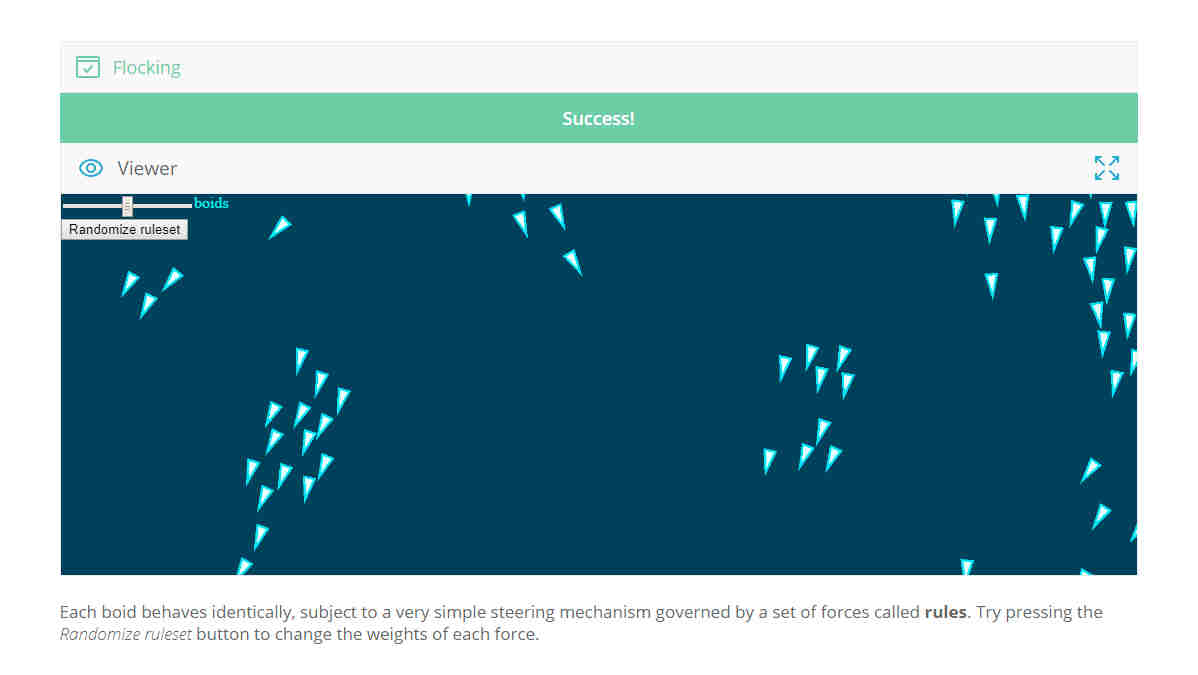
\includegraphics[width=\linewidth]{img/techio_game.jpg}
        \caption{A game developed and available in a \techio{} playground.}
    \end{subfigure}
    \hfill
    \begin{subfigure}{.45\linewidth}
        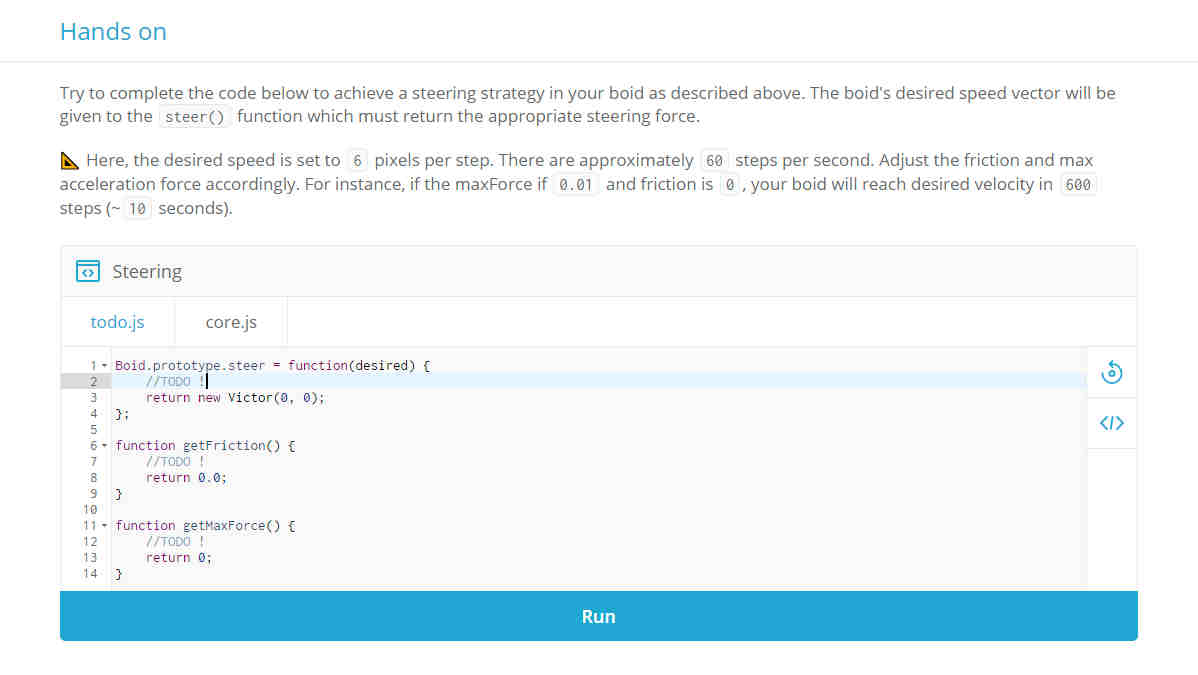
\includegraphics[width=\linewidth]{img/techio_handson.jpg}
        \caption{Coding in \techio.}
    \end{subfigure}
    \caption{Example pictures from \techio.}
\end{figure}

An investigation into alternative platforms to tech.io was launched. After some time of searching for a suitable alternative over the internet it was concluded that no platform really matched the requirements that were set. For the most part, only complete platforms with code verification were found that had closed APIs.

An example of such a platform would be code academy, which is an educational platform dedicated to providing the best learning experience for coding over the internet. However, it did not support individuals creating their own courses or using their code validation, hence it was not a viable candidate.
\begin{figure}[h]
   \centering
    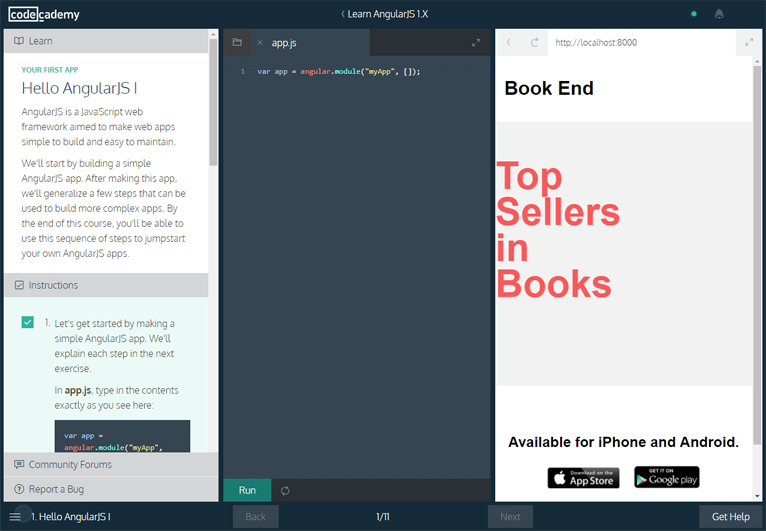
\includegraphics[width=.75\linewidth]{img/codeacademy_code.jpg}
    \caption{Example picture from codeacademy.}
\end{figure}


In contrast to \techio{}, a student at \LTU{} has developed an open platform called \sockr{} for hosting programming ladders. However, while the solution was more interesting from a licensing point of view, the source code of \sockr{} was mostly undocumented. It didn't have a clear API and the backend and frontend were too tightly coupled to be used in a sustainable way. It would require too much refactoring to be of use in the project.

After much research it was concluded that the best and most sustainable solution for the project would be to develop a code verification/compilation platform from scratch, effectively making the project completely independent of other services.
